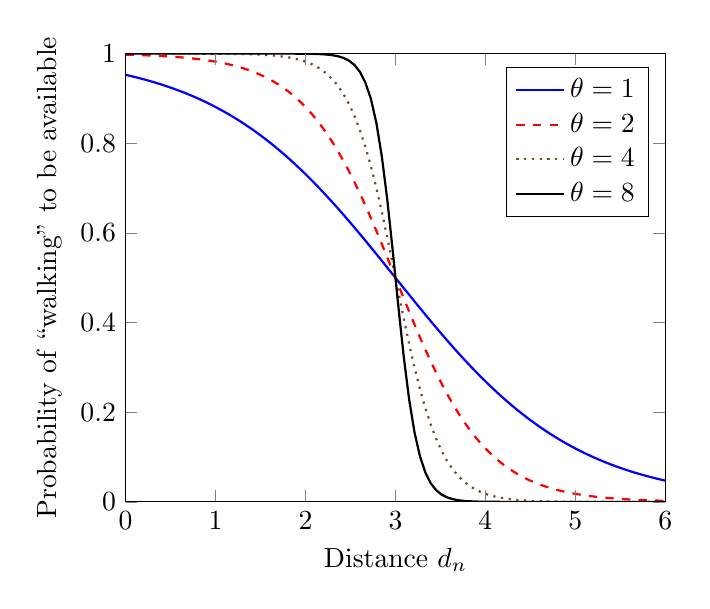
\begin{tikzpicture}[
  declare function = {
    f(\x,\theta) = 1 / (1 + exp(\theta*(\x - 3))) ;
  }
]
  \begin{axis}[
      xlabel={Distance $d_n$}, 
      ylabel={Probability of ``walking'' to be available}, 
      samples=100, 
      domain=0:6, 
      xmin=0, 
      xmax=6, 
      ymin=0, 
      ymax=1, 
      axis on top, 
      legend pos=north east, 
    ]
    \addplot+[no marks, thick] {f(x, 1)};
    \addlegendentry{$\theta=1$}
    \addplot+[no marks, thick, dashed] {f(x, 2)};
    \addlegendentry{$\theta=2$}
    \addplot+[no marks, thick, dotted] {f(x, 4)};
    \addlegendentry{$\theta=4$}
    \addplot+[no marks, thick] {f(x, 8)};
    \addlegendentry{$\theta=8$}
  \end{axis}
\end{tikzpicture}

